% !TeX program = xelatex
\documentclass[UTF8,11pt,fontset=fandol]{ctexart}
\usepackage[a4paper,left=18mm,right=18mm,top=17mm,bottom=16mm]{geometry}
\usepackage{graphicx,xcolor,amsmath,listings}
\usepackage[unicode,colorlinks=true]{hyperref}

\newcommand{\DocTitle}{基于GPT-6.2 Astra制作的六旋翼无人机}
\newcommand{\DocAuthors}{朱华天，GPT-6.2 Astra}
\newcommand{\DocDate}{2026年11月18日}
\newcommand{\RepoURL}{https://github.com/ZHT1235456/Three-js-Hexacopter-by-GPT-6.2-Astra}
\definecolor{ink}{HTML}{26353B}
\definecolor{muted}{HTML}{4C6065}
\definecolor{accent}{HTML}{A34921}
\definecolor{papergray}{HTML}{F0F3F2}
\hypersetup{pdftitle={\DocTitle},pdfauthor={\DocAuthors},pdflang={zh-CN},urlcolor=accent}
\setmainfont{TeX Gyre Termes}
\setsansfont{TeX Gyre Heros}
\setmonofont{Latin Modern Mono}[Scale=0.93]
\graphicspath{{figures/}{docs/figures/}}
\setlength{\parindent}{0pt}
\setlength{\parskip}{0pt}
\setlength{\abovedisplayskip}{4pt}
\setlength{\belowdisplayskip}{4pt}
\pagestyle{empty}
\raggedbottom
\newcommand{\topic}[1]{\par\vspace{3.2mm}{\heiti\sffamily\bfseries\fontsize{14}{18}\selectfont #1\par}\vspace{0.8mm}}
\newcommand{\photocaption}[2]{\par\vspace{1.1mm}{\raggedright\fontsize{9.2}{13}\selectfont
  {\heiti\sffamily\bfseries\color{accent}#1}\hspace{0.65em}{\color{muted}#2}\par}}
\lstset{basicstyle=\ttfamily\fontsize{10.2}{13}\selectfont,backgroundcolor=\color{papergray},
  columns=fullflexible,keepspaces=true,showstringspaces=false,upquote=true,
  frame=single,framerule=0pt,framesep=2mm,xleftmargin=2mm,xrightmargin=2mm,
  aboveskip=3mm,belowskip=0.8mm}

\begin{document}
\color{ink}
{\heiti\sffamily\bfseries\fontsize{23}{29}\selectfont\DocTitle\par}
\vspace{2mm}
{\sffamily\fontsize{11.2}{15}\selectfont\DocAuthors\par}
{\sffamily\fontsize{10.6}{14}\selectfont\DocDate\par}
{\fontsize{10}{14}\selectfont\href{\RepoURL}{\texttt{\RepoURL}}\par}
\vspace{2mm}
{\color{accent}\rule{\linewidth}{0.65pt}}\par
\vspace{2mm}

这款民用六旋翼用于航拍与教学展示。机壳和云台相机的造型参照了 ImageGen 生成的多视角部件图。一个可复用的 Three.js 模块在运行时生成整机几何、碳纤维纹理和镜片材质。
\par\vspace{3mm}

\noindent\begin{minipage}[t]{0.688\linewidth}
  \vspace{0pt}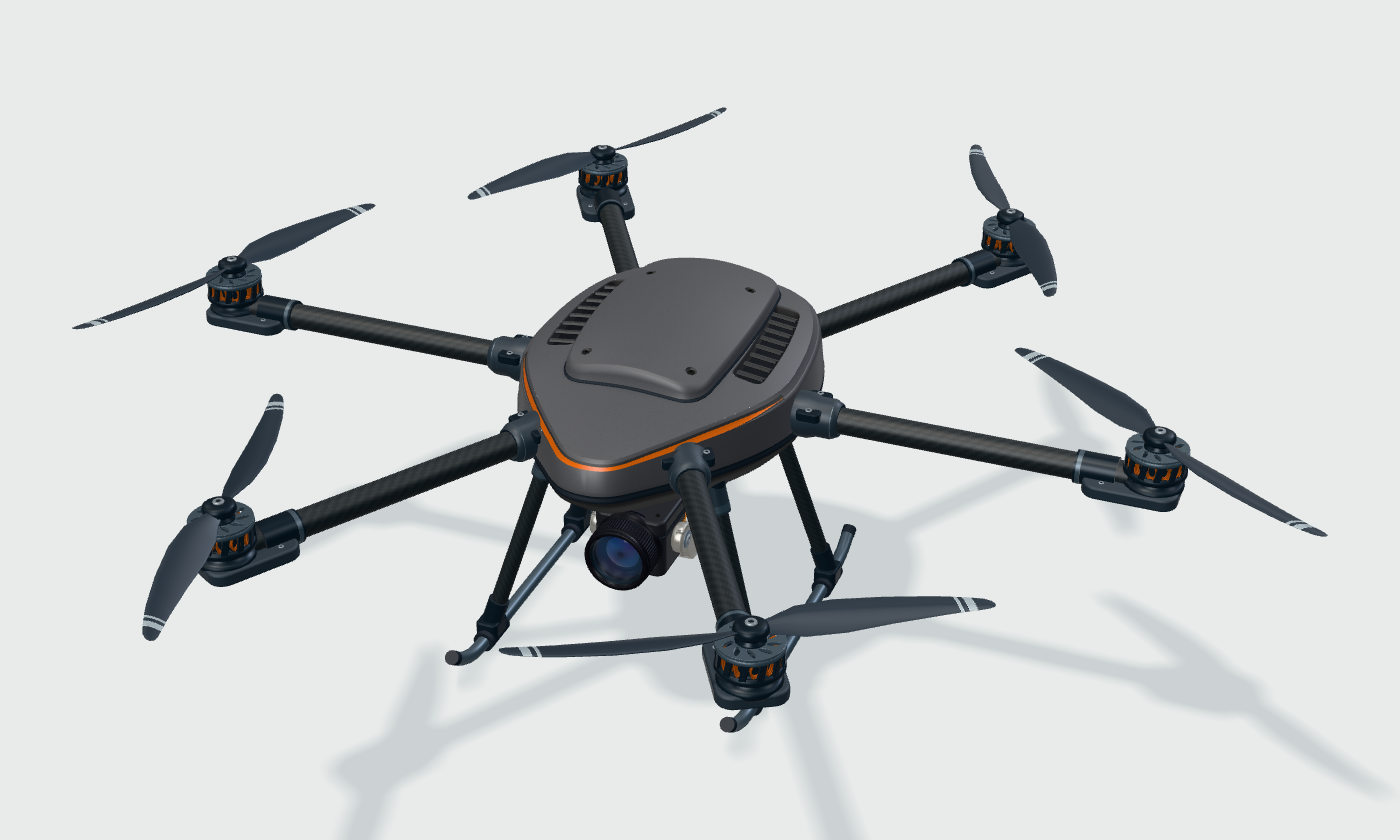
\includegraphics[width=\linewidth]{hexacopter.png}
  \photocaption{整机}{橙色嵌条勾出机头轮廓，航拍相机悬于双滑橇之间。}
\end{minipage}\hfill
\begin{minipage}[t]{0.287\linewidth}
  \vspace{0pt}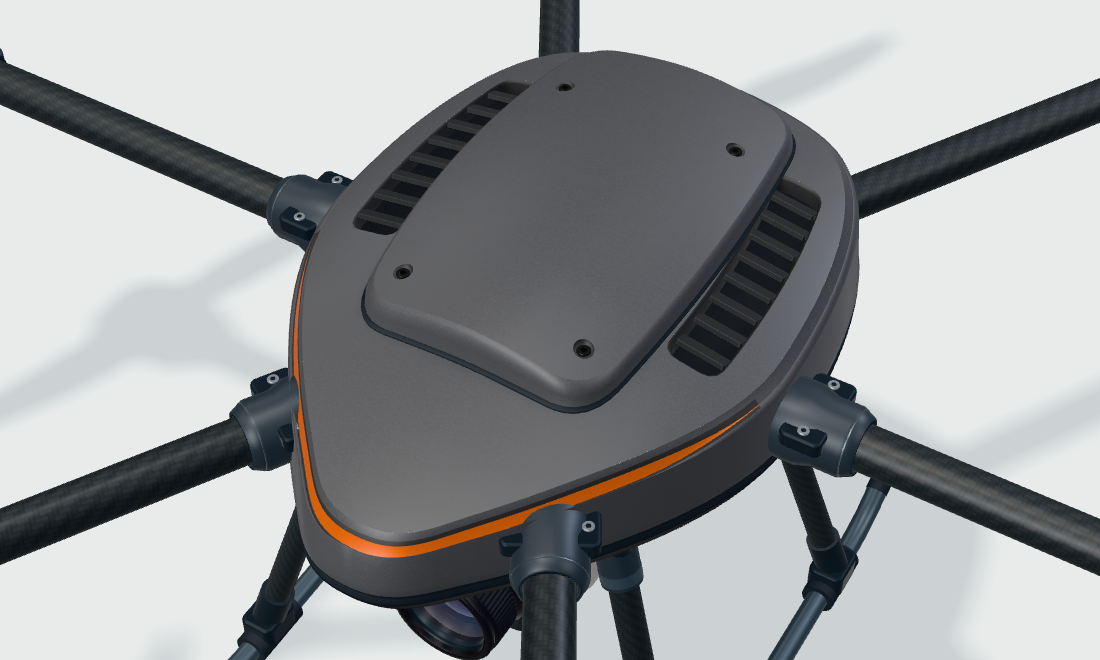
\includegraphics[width=\linewidth]{housing.png}
  \photocaption{机壳}{下沉百叶与沉头螺钉。}
  \vspace{2mm}
  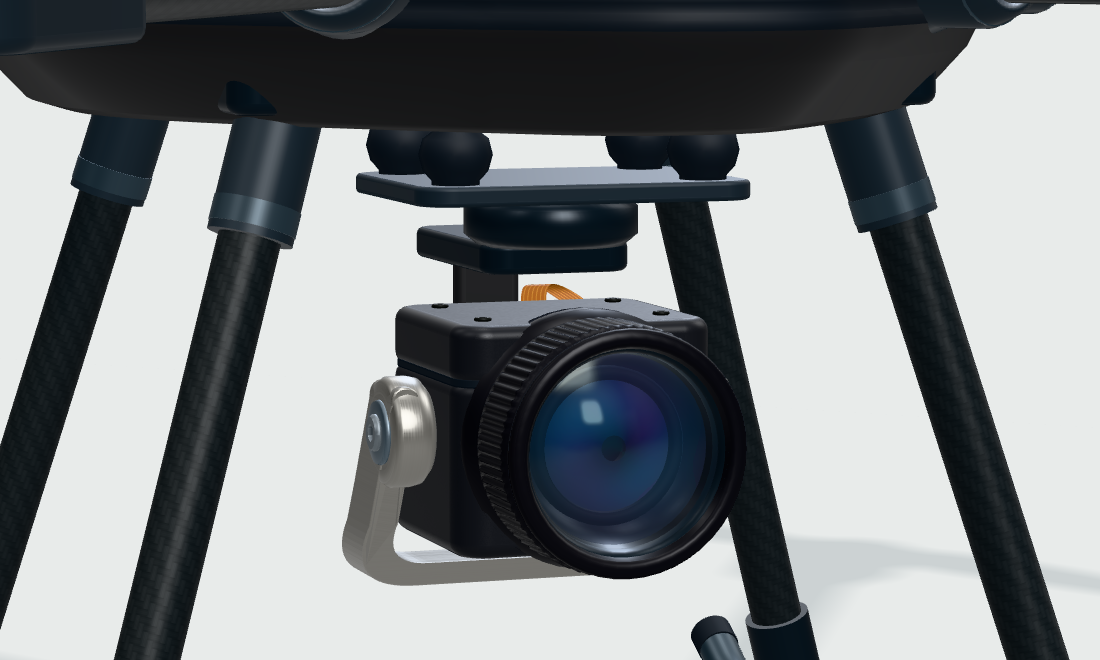
\includegraphics[width=\linewidth]{gimbal.png}
  \photocaption{云台}{弯折铝支架与镀膜镜片。}
\end{minipage}

\topic{机架几何}
模型以米为单位，原点位于双滑橇之间的地面上，\( +Y \) 向上，\( +Z \) 指向机头。六台电机等角分布在半径为 \(0.45\,\mathrm{m}\) 的圆上。将电机从 0 到 5 编号，轴心在水平面上的坐标为
\[
  \theta_i=\frac{\pi}{6}+i\frac{\pi}{3},\qquad
  (x_i,z_i)=(0.45\,\mathrm{m})(\sin\theta_i,\,\cos\theta_i),\qquad i=0,\ldots,5 .
\]
相邻机臂的夹角为 \(60^\circ\)，对置电机的轴距为 \(0.90\,\mathrm{m}\)，中央机壳最宽处为 \(0.27\,\mathrm{m}\)。从俯视图可见六根机臂的等角布局，从侧视图可见相机的悬挂位置与离地间隙。

\topic{旋翼动画与场景调用}
每副双叶桨都绕自身电机的局部 \(Y\) 轴旋转。\texttt{rotor-spin} 片段的演示速度为每秒一圈，相邻旋翼的转向相反。创建整机后，用 Three.js 的动画混合器播放该片段。
\begin{lstlisting}
const drone = createHexacopter();
scene.add(drone);
const mixer = new THREE.AnimationMixer(drone);
const clip = THREE.AnimationClip.findByName(drone.animations, 'rotor-spin');
mixer.clipAction(clip).play();
\end{lstlisting}
\vspace{1mm}
在渲染循环中调用 \texttt{mixer.update(dt)}，其中 \texttt{dt} 以秒计。相机俯仰由独立节点 \texttt{gimbal-pitch} 控制，绕局部 \(X\) 轴正向旋转时镜头下俯。
\end{document}
